\documentclass[12pt, a4paper]{report}
\usepackage{epsfig}
\usepackage{subfigure}
%\usepackage{amscd}
\usepackage{amssymb}
\usepackage{amsbsy}
\usepackage{amsmath}
\usepackage{amsthm}
\usepackage{framed}
\usepackage{subfiles}
%\usepackage[dvips]{graphicx}
\usepackage{natbib}
\bibliographystyle{chicago}
\usepackage{vmargin}
% left top textwidth textheight headheight
% headsep footheight footskip
\setmargins{3.0cm}{2.5cm}{15.5 cm}{22cm}{0.5cm}{0cm}{1cm}{1cm}
\renewcommand{\baselinestretch}{1.5}
\pagenumbering{arabic}
\theoremstyle{plain}
\newtheorem{theorem}{Theorem}[section]
\newtheorem{corollary}[theorem]{Corollary}
\newtheorem{ill}[theorem]{Example}
\newtheorem{lemma}[theorem]{Lemma}
\newtheorem{proposition}[theorem]{Proposition}
\newtheorem{conjecture}[theorem]{Conjecture}
\newtheorem{axiom}{Axiom}
\theoremstyle{definition}
\newtheorem{definition}{Definition}[section]
\newtheorem{notation}{Notation}
\theoremstyle{remark}
\newtheorem{remark}{Remark}[section]
\newtheorem{example}{Example}[section]
\renewcommand{\thenotation}{}
\renewcommand{\thetable}{\thesection.\arabic{table}}
\renewcommand{\thefigure}{\thesection.\arabic{figure}}
\title{Research notes: linear mixed effects models}
\author{ } \date{ }


\begin{document}
	\author{Kevin O'Brien}
	\title{Spring 2011}
	
	\addcontentsline{toc}{section}{Bibliography}
	
	\tableofcontents



%\section{Bartko's Bradley-Blackwood Test}
%
%\begin{itemize}
%	\item The Bradley Blackwood test is a simultaneous test for bias and
%	precision. They propose a regression approach which fits D on M,
%	where D is the difference and average of a pair of results.
%	\item Both beta values, the intercept and slope, are derived from the respective means and
%	standard deviations of their respective data sets.
%	\item We determine if the respective means and variances are equal if
%	both beta values are simultaneously equal to zero. The Test is
%	conducted using an F test, calculated from the results of a
%	regression of D on M.
%	\item We have identified this approach  to be examined to see if it can
%	be used as a foundation for a test perform a test on means and
%	variances individually.
%	\item Russell et al have suggested this method be used in conjunction
%	with a paired t-test , with estimates of slope and intercept.
%\end{itemize}
%subsection{t-test}


\chapter{Error In Variable Models}
\section{Regression Methods}
Conventional regression models are estimated using the ordinary least squares (OLS) technique, and are referred to as `Model I regression'\citep{CornCoch,ludbrook97}. A key feature of Model I models is that the independent variable is assumed to be measured
without error. As often pointed out in several papers \citep{BA83,ludbrook97}, this assumption invalidates simple linear
regression for use in method comparison studies, as both methods must be assumed to be measured with error.

The use of regression models that assumes the presence of error in both variables $X$ and $Y$ have been proposed for use instead.
\citep{CornCoch,ludbrook97}, These methodologies are collectively known as `Model II regression'. They differ in the method used to
estimate the parameters of the regression.

Regression estimates depend on formulation of the model. A formulation with one method considered as the $X$ variable will
yield different estimates for a formulation where it is the $Y$ variable. With Model I regression,the models fitted in both cases
will entirely different and inconsistent. However with Model II
regression, they will be consistent and complementary.

%------------------------------------------------------------------------------------------------------%

\section{Conclusions about Existing Methodologies}

Scatterplots are recommended by \citet{BA83} for an initial
examination of the data, facilitating an initial judgement and
helping to identify potential outliers. They are not useful for a
thorough examination of the data. \citet{BritHypSoc} notes that
data points will tend to cluster around the line of equality,
obscuring interpretation.


The Bland Altman methodology is well noted for its ease of use,
and can be easily implemented with most software packages. Also it
doesn't require the practitioner to have more than basic
statistical training. The plot is quite informative about the
variability of the differences over the range of measurements. For
example, an inspection of the plot will indicate the 'fan effect'.
They also can be used to detect the presence of an outlier.

\citet{ludbrook97,ludbrook02}criticizes these plots on the
basis that they presents no information on effect of constant bias
or proportional bias. These plots are only practicable when both
methods measure in the same units. Hence they are totally
unsuitable for conversion problems. The limits of agreement are
somewhat arbitrarily constructed. They may or may not be suitable
for the data in question. It has been found that the limits given
are too wide to be acceptable. There is no guidance on how to deal
with outliers. Bland and Altman recognize effect they would have
on the limits of agreeement, but offer no guidance on how to
correct for those effects.

There is no formal testing procedure provided. Rather, it is upon
the practitioner opinion to judge the outcome of the methodology.





%%%%%%%%%%%%%%%%%%%%%%%%%%%%%%%%%%%%%%%%%%%%%%%%%%%%%%%%%%%%%%%%%%%%%%%%%
%9 Appendix                  %%%%%%%%%%%%%%%%%%%%%%%%%%%%%%%%%%%%%%%%%%%%%
%%%%%%%%%%%%%%%%%%%%%%%%%%%%%%%%%%%%%%%%%%%%%%%%%%%%%%%%%%%%%%%%%%%%%%%%%



\section{Background} 
In method comparison studies, it is of importance to assure that the presence of a difference of medical importance is detected. 
For a given difference, the necessary number of samples depends on the range of values and the analytical standard deviations of the methods involved. For typical examples, the present study evaluates the statistical power of least-squares and Deming regression analyses applied to the method comparison data.

\section{Constant and Proportional Bias}

Linear Regression is a commonly used technique for comparing paired assays. The Intercept and Slope can provide estimates for the constant bias and proportional bias occurring between both methods. If the basic assumptions underlying linear regression are not met, the regression equation, and consequently the estimations
of bias are undermined. Outliers are a source of error in regression estimates.

Constant or proportional bias in method comparison studies using linear regression can be detected by an individual test on the intercept or the slope of the line regressed from the results of the two methods to be compared.

\begin{itemize}
	\item Model I regression
	\item Model II regression
\end{itemize}
Model I regression [Criterion v Test]
[Cornbleet Gochman 1979] define this analysis as the case in which the independent variable, X, is measured without error, with y as the dependent variable.

In method comparison studies, the X variable is a precisely measured reference method. In the [Cornbleet Gochman 1979] paper. It is argued that criterion may be regarded as the correct value. Other papers dispute this.


Model II regression [Test V Test]
In this type of analysis,both of the measurement methods are test methods, with both expected to be subject to error. Deming regression is an approach to model II regression.



Regression approaches are useful for a making a detailed examination of the biases across the range of measurements, allowing bias to be decomposed into fixed bias and proportional bias. Fixed bias describes the case where one method gives values that are consistently different to the other across the whole range. Proportional
bias describes the difference in measurements getting progressively greater, or smaller, across the range of measurements. A measurement method may have either an attendant fixed bias or proportional bias, or both. \citep{ludbrook}. Determination of these biases shall be discussed in due course.


\section{Cornbleet - Cochran }
This regression method also calculates a line of best fit for two sets of data. It differs from Model I regression in that it is derived in a way that factors in for error in the x-axis, as well as the y-axis. Cornbleet Gochman (1979) refer to it as 'Model II regression'.

\begin{itemize}
\item Model II regression [Test V Test] In this type of analysis,both of the measurement methods are test methods, with both expected to be subject to error. Deming regression is an approach to model II regression.

\item Model I regression [Criterion v Test] [Cornbleet Gochman 1979] define this analysis as the case in which the independent variable, X, is measured without error, with y as the dependent
variable.

\item In method comparison studies, the X variable is a precisely measured reference method. In the [Cornbleet Gochman 1979] paper It is argued that criterion may be regarded as the correct value.
Other papers dispute this.
\end{itemize}


%%%%%%%%%%%%%%%%%%%%%%%%%%%%%%%%%%%%%%%%%%%%%%%%%%%%%%%%%%%%%%%%%%%%%%%%%
%6 Regression Based Approaches          %%%%%%%%%%%%%%%%%%%%%%%%%%%%%%%%%
%%%%%%%%%%%%%%%%%%%%%%%%%%%%%%%%%%%%%%%%%%%%%%%%%%%%%%%%%%%%%%%%%%%%%%%%%




\section{Model I and II Regression}

On account of the fact that one set of measurements are linearly related to another, one could surmise that Linear Regression is the most suitable approach to analyzing comparisons. This approach is unsuitable on two counts. Firstly one of the assumptions of Regression analysis is that the independent variable values are without error. In method comparison studies one must assume the opposite; that there is error present in the measurements. Secondly a regression of X on Y would yield and entirely different result from Y on X.

Model I regression is unsuitable for method comparison studies. Even in the case where one method is a gold standard , it is disputed as to whether it is a valid approach. Model II regression is suitable for method comparison studies, but it is more difficult to execute. Both Model I and II regression models are unduly influenced by outliers.
Regression Models can not easily be used to analyze repeated measurements


Cochrane and Cornbleet argue for the use of methods that based on
the assumption that both methods are imprecisely measured ,and
that yield a fitting that is consistent with both '$X$ on $Y$' and
'$Y$ on $X$' formulations. These methods uses alternatives to the
OLS approach to determine the slope and intercept.

They describe three such alternative methods of regression; Deming, Mandel, and Bartlett regression. Collectively the authors refer to these approaches as Model II regression techniques.

\subsection{Model I regression [Criterion v Test]}
[Cornbleet Gochman 1979] define this analysis as the case in which the independent variable, X, is measured without error, with y as the dependent variable.
 
In method comparison studies, the X variable is a precisely measured reference method. In the [Cornbleet Gochman 1979] paper. It is argued that criterion may be regarded as the correct value. Other papers dispute this.
 

Simple Linear Regression is well known statistical technique, wherein estimates for slope and
intercept of the line of best fit are derived according to the Ordinary Least Square (OLS) principle. This method is known to Cornbleet and Cochrane as Model I regression.

Simple linear regression is defined as such with the name `Model I regression' by Cornbleet Gochman (1979), in contrast to 'Model II regression'.

 
\subsection{Model II regression [Test V Test]}
In this type of analysis, both of the measurement methods are test methods, with both expected to be subject to error. Deming regression is an approach to model II regression.



In Model I regression, the independent variable is assumed to be
measured without error. For method comparison studies, both sets of measurement must be assumed to be measured with imprecision and neither case can be taken to be a reference method. Arbitrarily
selecting either method as the reference will yield two conflicting outcomes. A fitting based on '$X$ on $Y$' will give inconsistent results with a fitting based on '$Y$ on $X$'. Consequently model I regression is inappropriate for such cases.


    % 1.A. Use of SLR, description of SLR as Model I
    % 1.B. Inappropriate for MCS
    % 1.C  Calibration and Conversion problems

 Simple linear regression is defined as such with the name `Model I regression' by Cornbleet Gochman (1979), in contrast to 'Model II regression'.

Simple linear regression calculates a line of best fit for two
sets of data, n which the independent variable, X, is measured without error, with y as the dependent variable.  

SLR (Model I) regression is considered by many \citet{BA83,CornCoch,ludbrook97} to be wholly unsuitable for
method comparison studies, although recommended for use in calibration studies [Corncoch]. Even in the case where one
method is a gold standard , it is disputed as to whether it is a valid approach. Model II regression is more suitable for method comparison studies, but it is more difficult to execute. Both Model I and II regression models are unduly influenced by outliers. Regression Models can not be used to analyze repeated measurements


Conventional regression models are estimated using the ordinary least squares (OLS) technique, and are referred to as `Model I regression'\citep{CornCoch,ludbrook97}. A key feature of Model I models is that the independent variable is assumed to be measured without error. As often pointed out in several papers \citep{BA83,ludbrook97}, this assumption invalidates simple linear
regression for use in method comparison studies, as both methods must be assumed to be measured with error.

The use of regression models that assumes the presence of error in both variables $X$ and $Y$ have been proposed for use instead. \citep{CornCoch,ludbrook97}, These methodologies are collectively known as `Model II regression'. They differ in the method used to
estimate the parameters of the regression.

Regression estimates depend on formulation of the model. A formulation with one method considered as the $X$ variable will
yield different estimates for a formulation where it is the $Y$ variable. With Model I regression,the models fitted in both cases
will entirely different and inconsistent. However with Model II
regression, they will be consistent and complementary.
\\
Conversely, Cornbleet Cochrane state that when the independent
variable $X$ is a precisely measured reference method, Model I
regression may be considered suitable. They qualify this statement
by referring the $X$ as \emph{the correct value}, tacitly
implying that there must still be some measurement error present.
The validity of this approach has been disputed elsewhere.

This regression method also calculates a line of best fit for two sets of data. It differs from Model I regression in that it is derived in a way that factors in for error in the x-axis, as well as the y-axis. Cornbleet Gochman (1979) refer to it as 'Model II regression'.

\subsection{Comparison of Model II regressions}
Cornbleet and Cochrane comparing the three methods, citing studies by other authors, concluding that Deming regression is the most useful of these methods. They found the Bartlett method to be
flawed in determining slopes.

However the author point out that \emph{ clinical laboratory measurements usually increase in absolute imprecision when larger values are measured.}However one of the assumptions that underline Deming and Mandel regression is constancy of the measurement errors throughout the range of values.

%\section{Advanced Regression Methods} In this section we examine some of the more advanced regression based approach employed in method comparison studies.

%\section{Variance components} Variance parameter must take an non-negative value. However an individual variance component, i.e. a component of the overall variance, may be negative.

%=========================================================================================== %



\section{Regression Methods}
	Conventional regression models are estimated using the ordinary
	least squares (OLS) technique, and are referred to as `Model I
	regression' \citep{CornCoch,ludbrook97}. A key feature of Model I
	models is that the independent variable is assumed to be measured
	without error. As often pointed out in several papers
	\citep{BA83,ludbrook97}, this assumption invalidates simple linear
	regression for use in method comparison studies, as both methods
	must be assumed to be measured with error.
	


%------------------------------------------------%



	


\section{Contention }
Several papers have commented that this approach is undermined
when the basic assumptions underlying linear regression are not
met, the regression equation, and consequently the estimations of
bias are undermined. Outliers are a source of error in regression
estimates.In method comparison studies, the X variable is a
precisely measured reference method. Cornbleet Gochman (1979)
argued that criterion may be regarded as the correct value. Other
papers dispute this.







\chapter{Errors-in-variables Regression}


% 1. SLR
% 2. EinV Regression
% 3. Deming Regression
% 4. Advanced Regression Methods



\section{Errors-in-variables models}

Errors-in-variables models or measurement errors models are regression models that account for measurement errors in the independent variables, as well as the dependent variable.

\section{Introduction}

Deming regression method also calculates a line of best fit for two sets of data. It differs from simple linear regression in that it is derived in a way that factors in for error in the x-axis, as
well as the y-axis.



%-----------------------------------------------------------------------------------------------%
\section{Origin of Deming Regression}
% %\citet{kummel}

Deming regression is a type of error-in-variable regression approach that assumes that the ratio $\lambda = \sigma^2_{epsilon}/\sigma^2_{\eta}$ is known. This approach would be appropriate when errors in $y$ and $x$ are both caused by measurements, and the accuracy of measuring devices or procedures are known. The case when $\lambda = 1$ is also known as the \textbf{\emph{orthogonal regression}}.

Deming regression is a regression fitting approach that assumes error in both variables.
The sum of squared distances from measured sets of values to the regression line is minimized at an angles specified by the ratio $\lambda$ of the residual variance of both variables. The variance of the ratio,$\lambda$, specifies the angle.  When $\lambda$ is one, the angle is 45 degrees. In ordinary linear regression, the distances are minimized in the vertical directions \citep{linnet99}.

As stated previously, the fundamental flaw of simple linear regression is that it allows for measurement error in one variable only. This causes a downward biased slope estimate.


The Deming regression method also calculates a line of best fit for two sets of data. Deming Regression differs from simple linear regression in that it is derived in a way that factors in for error in the x-axis, as well as the y-axis.

%-----------------------------------------------------------------------------------------------%

\section{Variance Ratio}
The Bland Altman Plot is uninformative about the comparative influence of proportional bias and fixed bias. Model II approaches, such as Deming regression,  can provide independent tests for
both types of bias.


As with conventional regression methodologies, Deming regression calculates an estimate for both the slope and intercept for the
fitted line, and standard errors thereof. Therefore there is sufficient information to carry out hypothesis tests on both
estimates, that are informative about presence of fixed and proportional bias.

\section{Bivariate Least Squares Regression} Since there
are errors in both methods, a regression technique that takes into account the individual errors in both axes (bivariate least-squares, BLS) should be used. In this paper, we demonstrate that the errors made in estimating the regression coefficients by the BLS method are fewer than with the ordinary least-squares (OLS) or weighted least-squares (WLS) regression techniques and that the coefficient can be considered normally distributed.

%================================================================================================= %

\section{Deming's Regression}
The most commonly known Model II methodology is known as Deming's Regression, (also known an Ordinary Least Product regression). Deming regression is recommended by \citet*{CornCoch} as the preferred Model II regression for use in method comparison studies. 

As previously noted, the Bland Altman Plot is
uninformative about the comparative influence of proportional bias and fixed bias. Deming's regression provides independent tests for both types of bias.


Deming regression method also calculates a line of best fit for two sets of data. It differs from simple linear regression in that it is derived in a way that factors in for error in the x-axis, as well as the y-axis.


\section{Deming Regression}
% - http://www.medcalc.org/manual/deming_regression.php
The Intercept and Slope are calculated according to Combleet \& Gochman, 1979. The standard errors and confidence intervals are estimated using the jackknife method (Armitage et al., 2002).
The 95\% confidence interval for the Intercept can be used to test the hypothesis that A=0. This hypothesis is accepted if the confidence interval for A contains the value 0. If the hypothesis is rejected, then it is concluded that A is significantly different from 0 and both methods differ at least by a constant amount.
The 95\% confidence interval for the Slope can be used to test the hypothesis that B=1. This hypothesis is accepted if the confidence interval for B contains the value 1. If the hypothesis is rejected, then it is concluded that B is significantly different from 1 and there is at least a proportional difference between the two methods.



\section{Deming Regression}

\begin{itemize}
	\item Informative analysis for the purposes of method comparison, Deming Regression is a regression technique taking into account uncertainty in both the independent and dependent variables.
	
	\item Deming’s method always results in one regression fit, regardless of which variable takes the place of the predictor variables.
	
	%Significant error in the least-squares slope estimation occurs when the ratio of the standard deviation of measurement of a single x value to the standard deviation of the indepedent variable data set exceeds 0.2.
	
	%Errors in the least-squares coefficients attributable to outliers can be avoided by eliminating data points whose vertical distance from the regression line exceed four times the standard error the estimate.
	
	\item The measurement error (lambda or $\lambda$) is specified with measurement error variance related as 
	\[\lambda = \sigma^2_y/\sigma^2_x\]
	
	(where $\sigma^2_x$ and $\sigma^2_y$ is the measurement error variance of the $x$ and $y$ variables, respectively).
	
	\item In the case where $\lambda$ is equal to one, (i.e. equal error variances), the methodology is equivalent to \textit{\textbf{orthogonal regression}}.
	
	\item Deming approaches the matter by simultaneously minimizing the sum of the square of the residuals of both variables. This derivation results in the best fit to minimize the sum of the squares of the perpendicular distances from the data points.
	
	\item To compute the slope by Deming’s formula,  normally distributed error of both variables  is assumed, as well as a constant level of imprecision throughout the range of measurements.
	
\end{itemize}

\section{Deming Regression}
Deming regression is a regression fitting approach that assumes error in both variables. Deming regression is recommended by \citet*{CornCoch} as the
preferred Model II regression for use in method comparison
studies. The sum of squared distances from measured sets of values to the regression line is minimized at an angles specified by the ratio $\lambda$ of the residual variance of both variables. 

The sum of squared distances from measured sets of values to the regression line is minimized at an angles specified by the ratio $\lambda$ of the residual variance of both variables. The variance of the ratio,$\lambda$, specifies the angle.  When $\lambda$ is one, the angle is 45 degrees. In ordinary linear regression, the distances are minimized in the vertical directions \citep{linnet99}.

As stated previously, the fundamental flaw of simple linear regression is that it allows for measurement error in one variable only. This causes a downward biased slope estimate.




When $\lambda$ is one, the angle is 45 degrees. In ordinary linear regression, the distances are minimized in the vertical directions \citep{linnet99}.
In cases involving only single measurements by each method, $\lambda$ may be unknown and is therefore assumes a value of one. While this will bias the estimates, it is less biased than ordinary linear regression.

%----------------------------------------------------------------------------------------------------

\section{Deming Regression}

The Deming regression line is estimated by minimizing the sums of squared deviations in both the x and y directions at an angle determined by the ratio of the analytical standard deviations for the two methods.

This ratio can be estimated if multiple measurements were taken with each method, but if only one measurement was taken with each method, it can be assumed to be equal to one.


\section{Deming Regression for MCS}
As noted before, Deming regression is an important and informative methodology in method comparison studies.
For single measurement method comparisons, Deming regression offers a useful complement to LME models.

\section{Drawbacks of Deming Regression}

Deming's Regression suffers from some crucial drawback. Firstly it is computationally complex, and it requires specific software packages to perform calculations. Secondly it is uninformative
about the comparative precision of two methods of measurement. Most importantly \citet{CarollRupert} states that

Deming's regression is acceptable only when the precision ratio ($\lambda$, in their paper as $\eta$) is correctly specified, but in practice this is often not the case, with the $\lambda$ being underestimated. This underestimation leads to an overcorrection for attenuation.

\section{Diagnostics for Deming Regression}
Model selection and diagnostic technique are well developed for classical linear regression methods.
Typically an implementation of a linear model fit will be accompanied by additional information, such as the coefficient of determination and likelihood and information criterions, and a regression ANOVA table. Such additional information has not, as yet, been implemented for Deming regression.



\section{Single measurements}
In cases involving only single measurements by each method, $\lambda$ may be unknown and is therefore assumes a value of one. While this will bias the estimates, it is less biased than ordinary linear regression.

%\citet{linnet93} defines analytical standard deviation as the standard deviation of measures values around the target value.\citet{linnet93} defines analytical standard deviation as the standard deviation of measures values around the target value.


\section{Performance in the presence of outliers}
All least square estimation methods are sensitive to outliers.
In common with all regression methods, Deming regression is vulnerable to outliers. 

Bland Altman's 1986 paper contains a data set, measurement of mean velocity of circumferential fibre shortening (VCF) by the long axis and short axis in M-mode echocardiography. Evident in this data set are outliers. Choosing the most noticeable, we shall use the deming regression method on this data set, both with and
without this outlier, to assess its influence.
\begin{itemize}
	\item In the presence of the outlier, the intercept and slope are estimated to be $-0.0297027$ and $1.0172959$ respectively.
	\item Without the outlier the intercept and slope are estimated to be
	$-0.11482220$ and  $1.09263112$ respectively.
	\item We therefore conclude that Deming Regression is adversely affected
	by outliers , in the same way model I regression is.
\end{itemize}

%------------------------------------------------%


\section{Deming Regression : Parameters and Estimation}


\subsection{RMSE} 


The root mean squared error is an estimate of the total error of the slope and includes the random error and the systemic error.

The root mean square error, RMSE,  is given by
\begin{equation*}
	\mbox{RMSE} = \sqrt{\sum{(b-1)^2/nruns}} =
	\sqrt{\mbox{(Bias)}^{2}+ \mbox{(SE)}^{2}}
\end{equation*}

where `nruns' is the number of runs.

\subsection{Estimating the Variance ratio}
\begin{eqnarray*}
	x_{i} = \mu +  \beta_{0} + \epsilon_{xi}\\
	y_{i} = \mu +  \beta_{1} + \epsilon_{yi}\\
\end{eqnarray*}
The inter-method bias is the difference of these biases. In order to determine an estimate for the residual variances, one of the method biases must be assumed to be zero, i.e. $\beta_{0} = 0$. The inter-method bias is now represented by $\beta_{1}$.

\begin{eqnarray*}
	x_{i} &=& \mu + \epsilon_{xi}\\
	y_{i} &=& \mu +  \beta_{1} + \epsilon_{yi}\\
\end{eqnarray*}

The residuals can be expressed as
\begin{eqnarray*}
	\epsilon_{xi} &=& x_{i} - \mu  \\
	\epsilon_{yi} &=& y_{i} - (\mu + \beta_{1}) \\
\end{eqnarray*}

The variance of the residuals are equivalent to the variance of the corresponding observations, $\sigma^{2}_{\epsilon x} =
\sigma^{2}_{x}$ and $\sigma^{2}_{\epsilon y} = \sigma^{2}_{y}$.
\begin{equation}
\lambda = \frac{\sigma^{2}_{yx}}{\sigma^{2}_{y}}.
\end{equation}

Assuming constant standard deviations, and given duplicate measurements, the analytical standard deviations are given by

\begin{eqnarray*}
	SD^{2}_{ax} = \frac{1}{2n} \sum (x_{2i} - x_{1i})^{2}\\
	SD^{2}_{ay} = \frac{1}{2n} \sum (y_{2i} - y_{1i})^{2}\\
\end{eqnarray*}



\section{Estimating the variance ratio (Linnet)}

Using duplicate measurements, one can estimate the analytical standard deviations and compute their ratio. This ratio is then used for computing the slope by the Deming method.[Linnet]

%----------------------------------------------------%


\section{Inference Procedures}
A $95\%$ confidence interval for the intercept estimate can be used to test the intercept, and hence fixed bias, is equal to
zero. This hypothesis is accepted if the confidence interval for the estimate contains the value $0$ in its range. Should this be,
it can be concluded that fixed bias is not present. Conversely, if the hypothesis is rejected, then it is concluded that the
intercept is non zero, and that fixed bias is present.

Testing for proportional bias is a very similar procedure. The $95\%$ confidence interval for the slope estimate can be used to
test the hypothesis that the slope is equal to $1$. This hypothesis is accepted if the confidence interval for the estimate
contains the value $1$ in its range. If the hypothesis is rejected, then it is concluded that the slope is significant
different from $1$ and that a proportional bias exists.

\begin{itemize}
	
	\item The 95\% confidence interval for the Intercept can be used to test the hypothesis that A=0. This hypothesis is accepted if the confidence interval for A contains the value 0. 
	\item If the hypothesis is rejected, then it is concluded that A is significant different from 0 and both methods differ at least by a constant amount. 
	
	\item The 95\% confidence interval for the Slope can be used to test the hypothesis that B=1. This hypothesis is accepted if the confidence interval for B contains the value 1. 
	
	\item If the hypothesis is rejected, then it is concluded that B is significant different from 1 and there is at least a proportional difference between the two methods. Cochrane Cornbleet
	\item The authors make the distinction between model I and model II regression types.
	\item Model II regression is the appropriate type when the predictor variable “x” is measured with imprecision.
	Cornbleet and Cochrane remark that clinical laboratory measurements usually increase in absolute imprecision when larger values are measured. % - [**]
\end{itemize}

%---------------------------------------------------------------------------------------%
A $95\%$ confidence interval for the intercept estimate can be used to test the intercept, and hence fixed bias, is equal to
zero. This hypothesis is accepted if the confidence interval for the estimate contains the value $0$ in its range. Should this be,
it can be concluded that fixed bias is not present. Conversely, if the hypothesis is rejected, then it is concluded that the
intercept is non zero, and that fixed bias is present.

Testing for proportional bias is a very similar procedure. The $95\%$ confidence interval for the slope estimate can be used to
test the hypothesis that the slope is equal to $1$. This hypothesis is accepted if the confidence interval for the estimate
contains the value $1$ in its range. If the hypothesis is rejected, then it is concluded that the slope is significant
different from $1$ and that a proportional bias exists.

\begin{itemize}
\item Model II regression is the appropriate type when the predictor variable “x” is measured with imprecision.
	Cornbleet and Cochrane remark that clinical laboratory measurements usually increase in absolute imprecision when larger values are measured. % - [**]
\end{itemize}

\subsubsection*{Guidelines}
Always plot the data. Suspected outliers may be identified from the scatter plot.
$S_{ex}$  represents the precision of a single x measurement near the mean value of X
\[\lambda = frac{S^2_{ex}}{S^2_{ey}}\]
%=========================================================================================================== %






\section{Using LME models to estimate the ratio (BXC) }

\begin{eqnarray*}
	y_{mi} &=& \mu + \beta_{m} + b_{i} + \epsilon_{mi}\\
\end{eqnarray*}

with $\beta_{m}$ is a fixed effect for the method $m$ and $b_{i}$ is a random effect associated with patient $i$, and
$\epsilon_{mi}$ as the measurement error. This is a simple single level LME model. \citet{pb} provides for the implementation of fitting a model. The variance ratio of the residual variances is immediately determinable from the output. This variance ratio can be use to fit a Deming regression, as described in chapter 1.




\section{Zhange Example}
For convenience, a new data set shall be introduced to demonstrate Deming regression. Measurements of transmitral volumetric flow (MF) by doppler echocardiography, and left ventricular stroke volume (SV) by cross sectional echocardiography in 21 patients
with aortic valve disease are tabulated in \citet{zhang}. This data set features in the discussion of method comparison studies
in \citet[p.398]{AltmanBook} .
%--------------------------------------------------------------------------------------------------------------%



% latex table generated in R 2.6.0 by xtable 1.5-5 package
% Tue Sep 01 13:31:17 2009
\begin{table}[h!]
	\begin{center}
		\begin{tabular}{|c|c|c||c|c|c||c|c|c|}
			\hline
			Patient & MF  & SV  & Patient & MF  & SV  & Patient & MF  & SV \\
			&($cm^{3}$)&  ($cm^{3}$) & &($cm^{3}$)&  ($cm^{3}$) & &($cm^{3}$)&  ($cm^{3}$)
			\\
			\hline
			1 & 47 & 43 &  8 & 75 & 72 &  15 & 90 & 82 \\
			2 & 66 & 70 & 9 & 79 & 92 &  16 & 100 & 100 \\
			3 & 68 & 72 & 10 & 81 & 76 & 17 & 104 & 94 \\
			4 & 69 & 81 & 11 & 85 & 85 &  18 & 105 & 98 \\
			5 & 70 & 60 & 12 & 87 & 82 & 19 & 112 & 108 \\
			6 & 70 & 67 & 13 & 87 & 90 & 20 & 120 & 131 \\
			7 & 73 & 72 & 14 & 87 & 96 &  21 & 132 & 131 \\
			
			\hline
		\end{tabular}
		\caption{Transmitral volumetric flow(MF) and left ventricular
			stroke volume (SV) in 21 patients. (Zhang et al 1986)}
	\end{center}
\end{table}

\begin{figure}[h!]
	% Requires \usepackage{graphicx}
	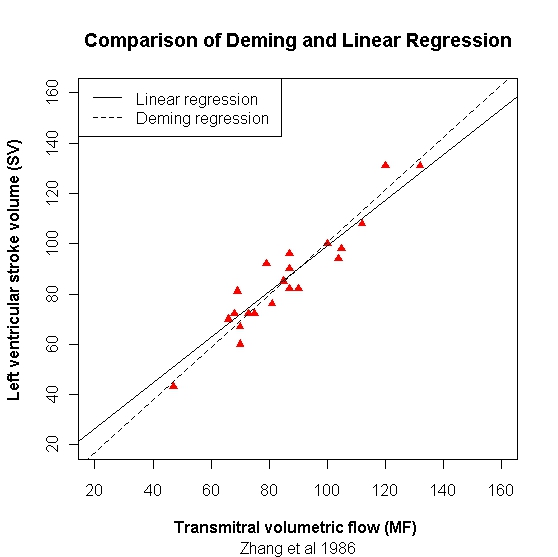
\includegraphics[width=130mm]{images/ZhangDeming.jpeg}
	\caption{Deming Regression For Zhang's Data}\label{ZhangDeming}
\end{figure}


\newpage



%============================================================================================= %
\section{Kummel's Estimates}
For a given $\lambda$, \citet{Kummel} derived the following estimate that would later be used for the Deming regression slope
parameter. The intercept estimate $\alpha$ is simply estimated in the same way as in conventional linear
regression, by using the identity $\bar{Y}-\hat{\beta}\bar{X}$;
\begin{equation}
	\hat{\beta} =\quad \frac{S_{yy} - \lambda S_{xx}+[(S_{yy} -
		\lambda S_{xx})^{2}+ 4\lambda S^{2}_{xy}]^{1/2}}{2S_{xy}}
\end{equation},
with $\lambda$ as the variance ratio. As stated previously $\lambda$ is often unknown, and therefore must be assumed to equal one. 

For a given $\lambda$, \citet{Kummel} derived the following estimate that would later be used for the Deming regression slope
parameter. The intercept estimate $\alpha$ is simply estimated in the same way as in conventional linear
regression, by using the identity $\bar{Y}-\hat{\beta}\bar{X}$;
\begin{equation}
	\hat{\beta} =\quad \frac{S_{yy} - \lambda S_{xx}+[(S_{yy} -
		\lambda S_{xx})^{2}+ 4\lambda S^{2}_{xy}]^{1/2}}{2S_{xy}}
\end{equation},
with $\lambda$ as the variance ratio. As stated previously $\lambda$ is often unknown, and therefore must be assumed to equal one. 

\citet{CarollRupert} states that Deming
regression is acceptable only when the precision ratio ($\lambda$,in their paper as $\eta$) is correctly specified, but in practice this is often not the case, with the $\lambda$ being underestimated. Several candidate models, with varying variance ratios may be fitted, and estimates of the slope and intercept are produced. However no model selection information is available to determine the best fitting model.

As with conventional regression methodologies, Deming regression calculates an estimate for both the slope and intercept for the
fitted line, and standard errors thereof. Therefore there is sufficient information to carry out hypothesis tests on both
estimates, that are informative about presence of fixed and proportional bias.

%---------------------------------------------------------------------------------------%
A $95\%$ confidence interval for the intercept estimate can be used to test the intercept, and hence fixed bias, is equal to
zero. This hypothesis is accepted if the confidence interval for the estimate contains the value $0$ in its range. Should this be,
it can be concluded that fixed bias is not present. Conversely, if the hypothesis is rejected, then it is concluded that the
intercept is non zero, and that fixed bias is present.

Testing for proportional bias is a very similar procedure. The
$95\%$ confidence interval for the slope estimate can be used to
test the hypothesis that the slope is equal to $1$. This
hypothesis is accepted if the confidence interval for the estimate
contains the value $1$ in its range. If the hypothesis is
rejected, then it is concluded that the slope is significant
different from $1$ and that a proportional bias exists.



% Koning
% http://www.springerlink.com/content/r1063462u618q483/

\begin{verbatim}
Use of deming regression in method comparison studies.
Henk Konings
\end{verbatim}

Accuracy is closeness to the true value, or alternatively, having a low measurement error.

The determination of a true value for a biological specimen is difficult and sometimes impossible.

Precision is expressed in terms of standard deviation, coefficient of variance or variance.

In Deming regression, the errors between methods are assigned to both methods in proportion to the variances of the methods.





\section{Implementations}
Thus far, one of the few \texttt{R} implementations of Deming regression is contained in the `MethComp' package. \citep{BXC2008}.

Unless specified otherwise, the variance ratio $\lambda$ has a default value of one. A means of computing likelihood functions would potentially allow for an algorithm for estimating the true variance ratio.


\section{Performance in the presence of outliers}
All least square estimation methods are sensitive to outliers.
In common with all regression methods, Deming regression is vulnerable to outliers. 

Bland Altman's 1986 paper contains a data set, measurement of mean velocity of circumferential fibre shortening (VCF) by the long axis and short axis in M-mode echocardiography. Evident in this data set are outliers. Choosing the most noticeable, we shall use the deming regression method on this data set, both with and
without this outlier, to assess its influence.
\begin{itemize}
	\item In the presence of the outlier, the intercept and slope are estimated to be $-0.0297027$ and $1.0172959$ respectively.
	\item Without the outlier the intercept and slope are estimated to be
	$-0.11482220$ and  $1.09263112$ respectively.
	\item We therefore conclude that Deming Regression is adversely affected
	by outliers , in the same way model I regression is.
\end{itemize}


%------------------------------------------------%



\section{Using LMEs to estimate the ratio}

\begin{eqnarray*}
	y_{mi} &=& \mu + \beta_{m} + b_{i} + \epsilon_{mi}
\end{eqnarray*}

with $\beta_{m}$ is a fixed effect for the method $m$ and $b_{i}$
is a random effect associated with patient $i$, and
$\epsilon_{mi}$ as the measurement error.

This is a simple single level LME model. \citet{pb} provides for
the implementation of fitting a model.

The variance ratio of the residual variances is immediately
determinable from the output. This variance ratio can be use to
fit a Deming regression, as described in chapter 1.


%------------------------------------------------------------------------------------%


\section{Least Products Regression}
Used as an alternative to Bland-Altman Analysis, this method is also known as 'Geometric Mean Regression' and 'Reduced Major Axis Regression'. This regression model minimizes the areas of the right triangles formed by the data points' vertical and horizontal deviations from the fitted line and the fitted line.

\begin{itemize}
	\item Model II regression analysis caters for cases in which random error is attached to both dependent and independent variables. Comparing methods of measurement is just such a case.(Ludbrook)
	
	\item Least products regression is the reviewer's preferred technique for analysing the Model II case. In this, the sum of the products of the vertical and horizontal deviations of the x,y values from the line is minimized.
	
	\item Least products regression analysis is suitable for calibrating one method against another. It is also a sensitive technique for detecting and distinguishing fixed and proportional bias between
	methods.
\end{itemize}

Least-products regression can lead to inflated SEEs and estimates that do not tend to their true values an N approaches infinity (Draper and Smith, 1998).







\section{Deming Regression}

\begin{itemize}
	\item Informative analysis for the purposes of method comparison, Deming Regression is a regression technique taking into account uncertainty in both the independent and dependent variables.
	
	\item Deming’s method always results in one regression fit, regardless of which variable takes the place of the predictor variables.
	
	%Significant error in the least-squares slope estimation occurs when the ratio of the standard deviation of measurement of a single x value to the standard deviation of the indepedent variable data set exceeds 0.2.
	
	%Errors in the least-squares coefficients attributable to outliers can be avoided by eliminating data points whose vertical distance from the regression line exceed four times the standard error the estimate.
	
	\item The measurement error (lambda or $\lambda$) is specified with measurement error variance related as 
	\[\lambda = \sigma^2_y/\sigma^2_x\]
	
	(where $\sigma^2_x$ and $\sigma^2_y$ is the measurement error variance of the $x$ and $y$ variables, respectively).
	
	\item In the case where $\lambda$ is equal to one, (i.e. equal error variances), the methodology is equivalent to \textit{\textbf{orthogonal regression}}.
	
	\item Deming approaches the matter by simultaneously minimizing the sum of the square of the residuals of both variables. This derivation results in the best fit to minimize the sum of the squares of the perpendicular distances from the data points.
	
	\item To compute the slope by Deming’s formula,  normally distributed error of both variables  is assumed, as well as a constant level of imprecision throughout the range of measurements.
	
\end{itemize}
\newpage
\section{Deming Regression- Line of Best Fit}


Deming regression method also calculates a line of best fit for two sets of data. It differs from simple linear regression in that it is derived in a way that factors in for error in the x-axis, as
well as the y-axis.




\section{Using LMEs to estimate the ratio}

\begin{eqnarray*}
	y_{mi} &=& \mu + \beta_{m} + b_{i} + \epsilon_{mi}\\
\end{eqnarray*}

with $\beta_{m}$ is a fixed effect for the method $m$ and $b_{i}$
is a random effect associated with patient $i$, and
$\epsilon_{mi}$ as the measurement error.

This is a simple single level LME model. \citet{pb} provides for
the implementation of fitting a model.

The variance ratio of the residual variances is immediately
determinable from the output. This variance ratio can be use to
fit a Deming regression, as described in chapter 1.




%=================================================================================================== %


\section{Methods} 
Theoretical calculations and simulations were used to consider the statistical power for detection of slope deviations from 
unity and intercept deviations from zero. For situations with proportional analytical standard deviations, weighted forms of regression analysis were evaluated.

\section{Results} In general, sample sizes of 40–100 samples conventionally used in method comparison studies often must 
be reconsidered. A main factor is the range of values, which should be as wide as possible for the given analyte. 
For a range ratio (maximum value divided by minimum value) of 2, 544 samples are required to detect one standardized slope 
deviation; the number of required samples decreases to 64 at a range ratio of 10 (proportional analytical error). For electrolytes having very narrow ranges of values, very large sample sizes usually are necessary. In case of proportional analytical error, application of a weighted approach is important to assure an efficient analysis; e.g., for a range ratio of 10, the weighted approach reduces the requirement of samples by >50%.

\section{Conclusions} Estimation of the necessary sample size for a method comparison study assures a valid result; either no difference is found or the existence of a relevant difference is confirmed.






\section{Weighted Deming Regression}
Weighted linear regression allows for non-constancy of the standard deviation of the $y$ variable. However it is assumed that $X$ is without measurement error. Weighted Deming regression takes into account the non-constant proportional measurement errors in both variables.Despite the non-constancy, it is necessary to retain the constant value of $\lambda$.

In \textbf{both forms} of Deming regression, $\lambda$ is assumed to be constant through out the range of measurements. For WDR weights $w_{i}$ are used to compute the sums of squares and cross products. The weights are inversely proportional to the squared analytical variance at any given value.



\section{Least Product Regression}

\begin{itemize}
	\item Least Product Regression , also known as 'Model II regression'
	caters for cases in which random error is attached to both
	dependent and independent variables. Ludbrook cites this
	methodology as being pertinent to Method comparison studies.
	
	\item 
	The sum of the products of the vertical and horizontal deviations
	of the x,y values from the line is minimized.
	
	\item 
	Least products regression analysis is considered suitable for
	calibrating one method against another.Ludbrook comments that it
	is also a sensitive technique for detecting and distinguishing
	fixed and proportional bias between methods.
	
	\item 
	Proposed as an alternative to Bland \& Altman methodology ,this
	method is also known as 'Geometric Mean Regression' and 'Reduced
	Major Axis Regression'.
\end{itemize}
%%------------------------------------------------------------------------------------%%





\section{Least Products Regression}
Used as an alternative to Bland-Altman Analysis, this method is also known as 'Geometric Mean Regression' and 'Reduced Major Axis Regression'. This regression model minimizes the areas of the right triangles formed by the data points' vertical and horizontal deviations from the fitted line and the fitted line.

\begin{itemize}
	\item Model II regression analysis caters for cases in which random error is attached to both dependent and independent variables. Comparing methods of measurement is just such a case.(Ludbrook)
	
	\item Least products regression is the reviewer's preferred technique for analysing the Model II case. In this, the sum of the products of the vertical and horizontal deviations of the x,y values from the line is minimized.
	
	\item Least products regression analysis is suitable for calibrating one method against another. It is also a sensitive technique for detecting and distinguishing fixed and proportional bias between
	methods.
\end{itemize}

Least-products regression can lead to inflated SEEs and estimates that do not tend to their true values an N approaches infinity (Draper and Smith, 1998).

\subsubsection{Difference with Least Squares Regression}
Least-products regression can lead to inflated SEEs and estimates
that do not tend to their true values an N approaches infinity
(Draper and Smith, 1998).




\section{Linnet - References}
The statistical procedures are described in:
Linnet K. Necessary sample size for method comparison studies based on regression analysis. Clin Chem 1999; 45: 882-94.
Linnet K. Performance of Deming regression analysis in case of misspecified analytical error ratio in method comparison studies. Clin Chem 1998; 44: 1024-1031.
Linnet K. Evaluation of regression procedures for methods comparison studies. Clin Chem 1993; 39. 424-432.
Linnet K. Estimation of the linear relationship between measurements of two methods with proportional errors. Stat Med 1990; 9: 1463-1473.

\section{Drawbacks}
Deming's Regression suffers from some crucial drawback. Firstly it
is computationally complex, and it requires specific software
packages to perform calculations.Secondly it is uninformative
about the comparative precision of two methods of measurement.
Most importantly \citet{CarollRupert} states that Deming's
regression is acceptable only when the precision ratio ($\lambda$,
in their paper as $\eta$) is correctly specified ,but in practice
this is often not the case, with the $\lambda$ being
underestimated.	
%-----------------------------------------%


\section{Bootstap Techniques}
Use of Bootstap Techniques to obtain Confidence Interval estimates

\section{References}
Carpenter, J., Bithell, J. (2000) Bootstrap confidence intervals: when, which, what? A practical
guide for medical statisticians. Stat Med, 19 (9), 1141–1164.

%============================================================================= %



\section{Estimating the Variance ratio}
\begin{eqnarray*}
	x_{i} = \mu +  \beta_{0} + \epsilon_{xi}\\
	y_{i} = \mu +  \beta_{1} + \epsilon_{yi}\\
\end{eqnarray*}
The inter-method bias is the difference of these biases. In order to determine an estimate for the residual variances, one of the method biases must be assumed to be zero, i.e. $\beta_{0} = 0$. The inter-method bias is now represented by $\beta_{1}$.

\begin{eqnarray*}
	x_{i} &=& \mu + \epsilon_{xi}\\
	y_{i} &=& \mu +  \beta_{1} + \epsilon_{yi}\\
\end{eqnarray*}

The residuals can be expressed as
\begin{eqnarray*}
	\epsilon_{xi} &=& x_{i} - \mu  \\
	\epsilon_{yi} &=& y_{i} - (\mu + \beta_{1}) \\
\end{eqnarray*}

The variance of the residuals are equivalent to the variance of the corresponding observations, $\sigma^{2}_{\epsilon x} =
\sigma^{2}_{x}$ and $\sigma^{2}_{\epsilon y} = \sigma^{2}_{y}$.
\begin{equation}
\lambda = \frac{\sigma^{2}_{yx}}{\sigma^{2}_{y}}.
\end{equation}

Assuming constant standard deviations, and given duplicate measurements, the analytical standard deviations are given by

\begin{eqnarray*}
	SD^{2}_{ax} = \frac{1}{2n} \sum (x_{2i} - x_{1i})^{2}\\
	SD^{2}_{ay} = \frac{1}{2n} \sum (y_{2i} - y_{1i})^{2}\\
\end{eqnarray*}

Using duplicate measurements, one can estimate the analytical
standard deviations and compute their ratio. This ratio is then
used for computing the slope by the Deming method.[Linnet]

\section{determining lambda}
assuming constant standard deviations, and given duplicate
measurements, the analytical standard deviations are given by

\begin{eqnarray*}
	SD^{2}_{ax} = \frac{1}{2n} \sum (x_{2i} - x_{1i})^{2}\\
	SD^{2}_{ay} = \frac{1}{2n} \sum (y_{2i} - y_{1i})^{2}\\
\end{eqnarray*}

%\section{performance in the presence of oultiers}
%All least square estimation methods are sensitive to outliers.

\section{weighted least square regression}
The constancy of variance is a necessary assumption for ordinary
linear regression.

\begin{equation}
	\mbox{SD}_{ay}  = ch(x_{i})
\end{equation}

\section{Weighted Deming Regression}

Weighted linear regression allows for non-constancy of the standard deviation of the $y$ variable. However it is assumed that $X$ is without measurement error. Weighted Deming regression takes into account the non-constant proportional measurement errors in both variables.Despite the non-constancy, it is necessary to retain the constant value of $\lambda$.

In \textbf{both forms} of Deming regression, $\lambda$ is assumed to be constant through out the range of measurements. For WDR weights $w_{i}$ are used to compute the sums of squares and cross products. The weights are inversely proportional to the squared analytical variance at any given value.






\section{Ordinary Least Product Regression}
\citet{ludbrook97} states that the grouping structure can be
straightforward, but there are more complex data sets that have a hierarchical(nested) model.

Observations between groups are independent, but observations
within each groups are dependent because they belong to the same
subpopulation. Therefore there are two sources of variation:
between-group and within-group variance.
 \vspace{5 mm} \noindent Mean correction is a method of reducing
bias.
%-------------------------------------------------



\end{document}
